\section{Сохранение иллюстрации}

После всех манипуляций мы получили иллюстрацию, которую нужно сохранить, во-первых, в формате изображения, пригодного для вставки в презентацию или статью, а, во вторых, во внутреннем формате химеры, на случай, если вы захотите что-то поменять в будущем.

\subsection*{Задание~8}
\begin{enumerate}
    \item Сохраните сессию:\\
    \texttt{File~> Save session as \dots}
    
    \item Экспортируйте сцену как изображение в формате PNG:\\
    \texttt{File~> Save Image}
    
    \item Попробуйте разные алгоритмы рендера (Chimera / POV-ray). В чем разница?
\end{enumerate}

\begin{figure}
\begin{subfigure}{.5\textwidth}
  \centering
  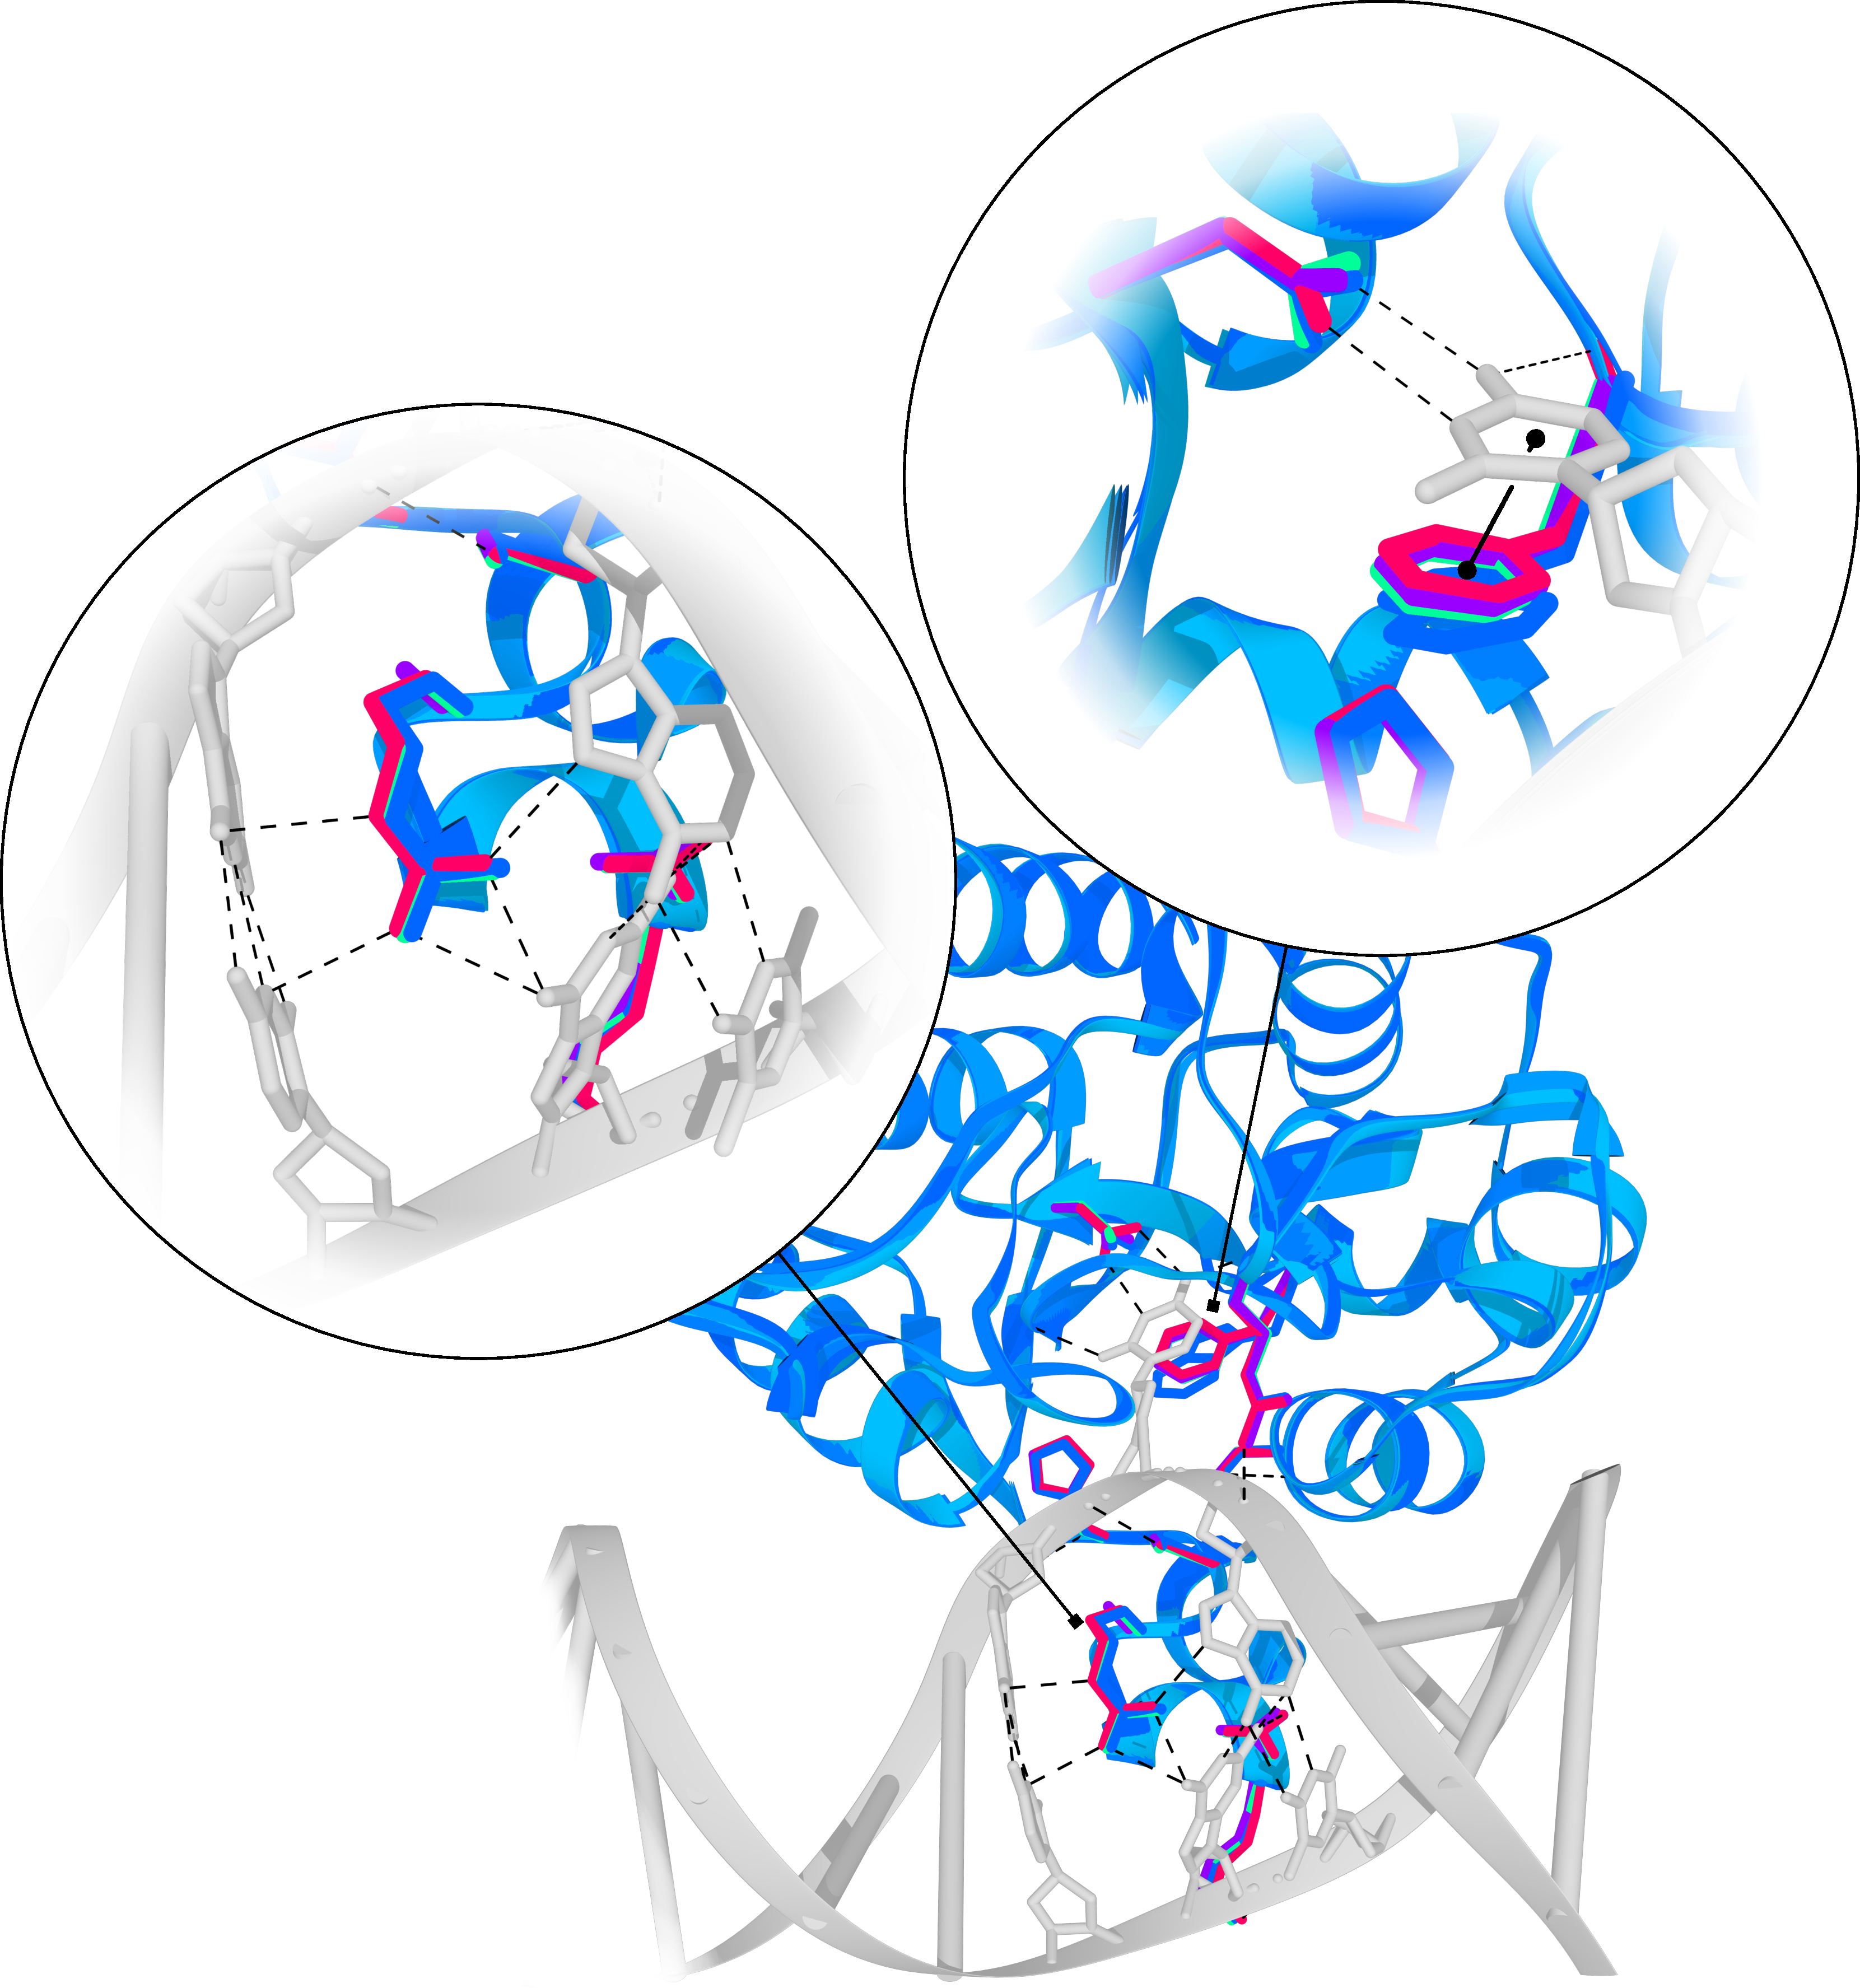
\includegraphics[width=.8\linewidth]{Guide/Figures/Protein.pdf}
  \caption{1a}
  \label{fig:sfig1}
\end{subfigure}%
\begin{subfigure}{.5\textwidth}
  \centering
  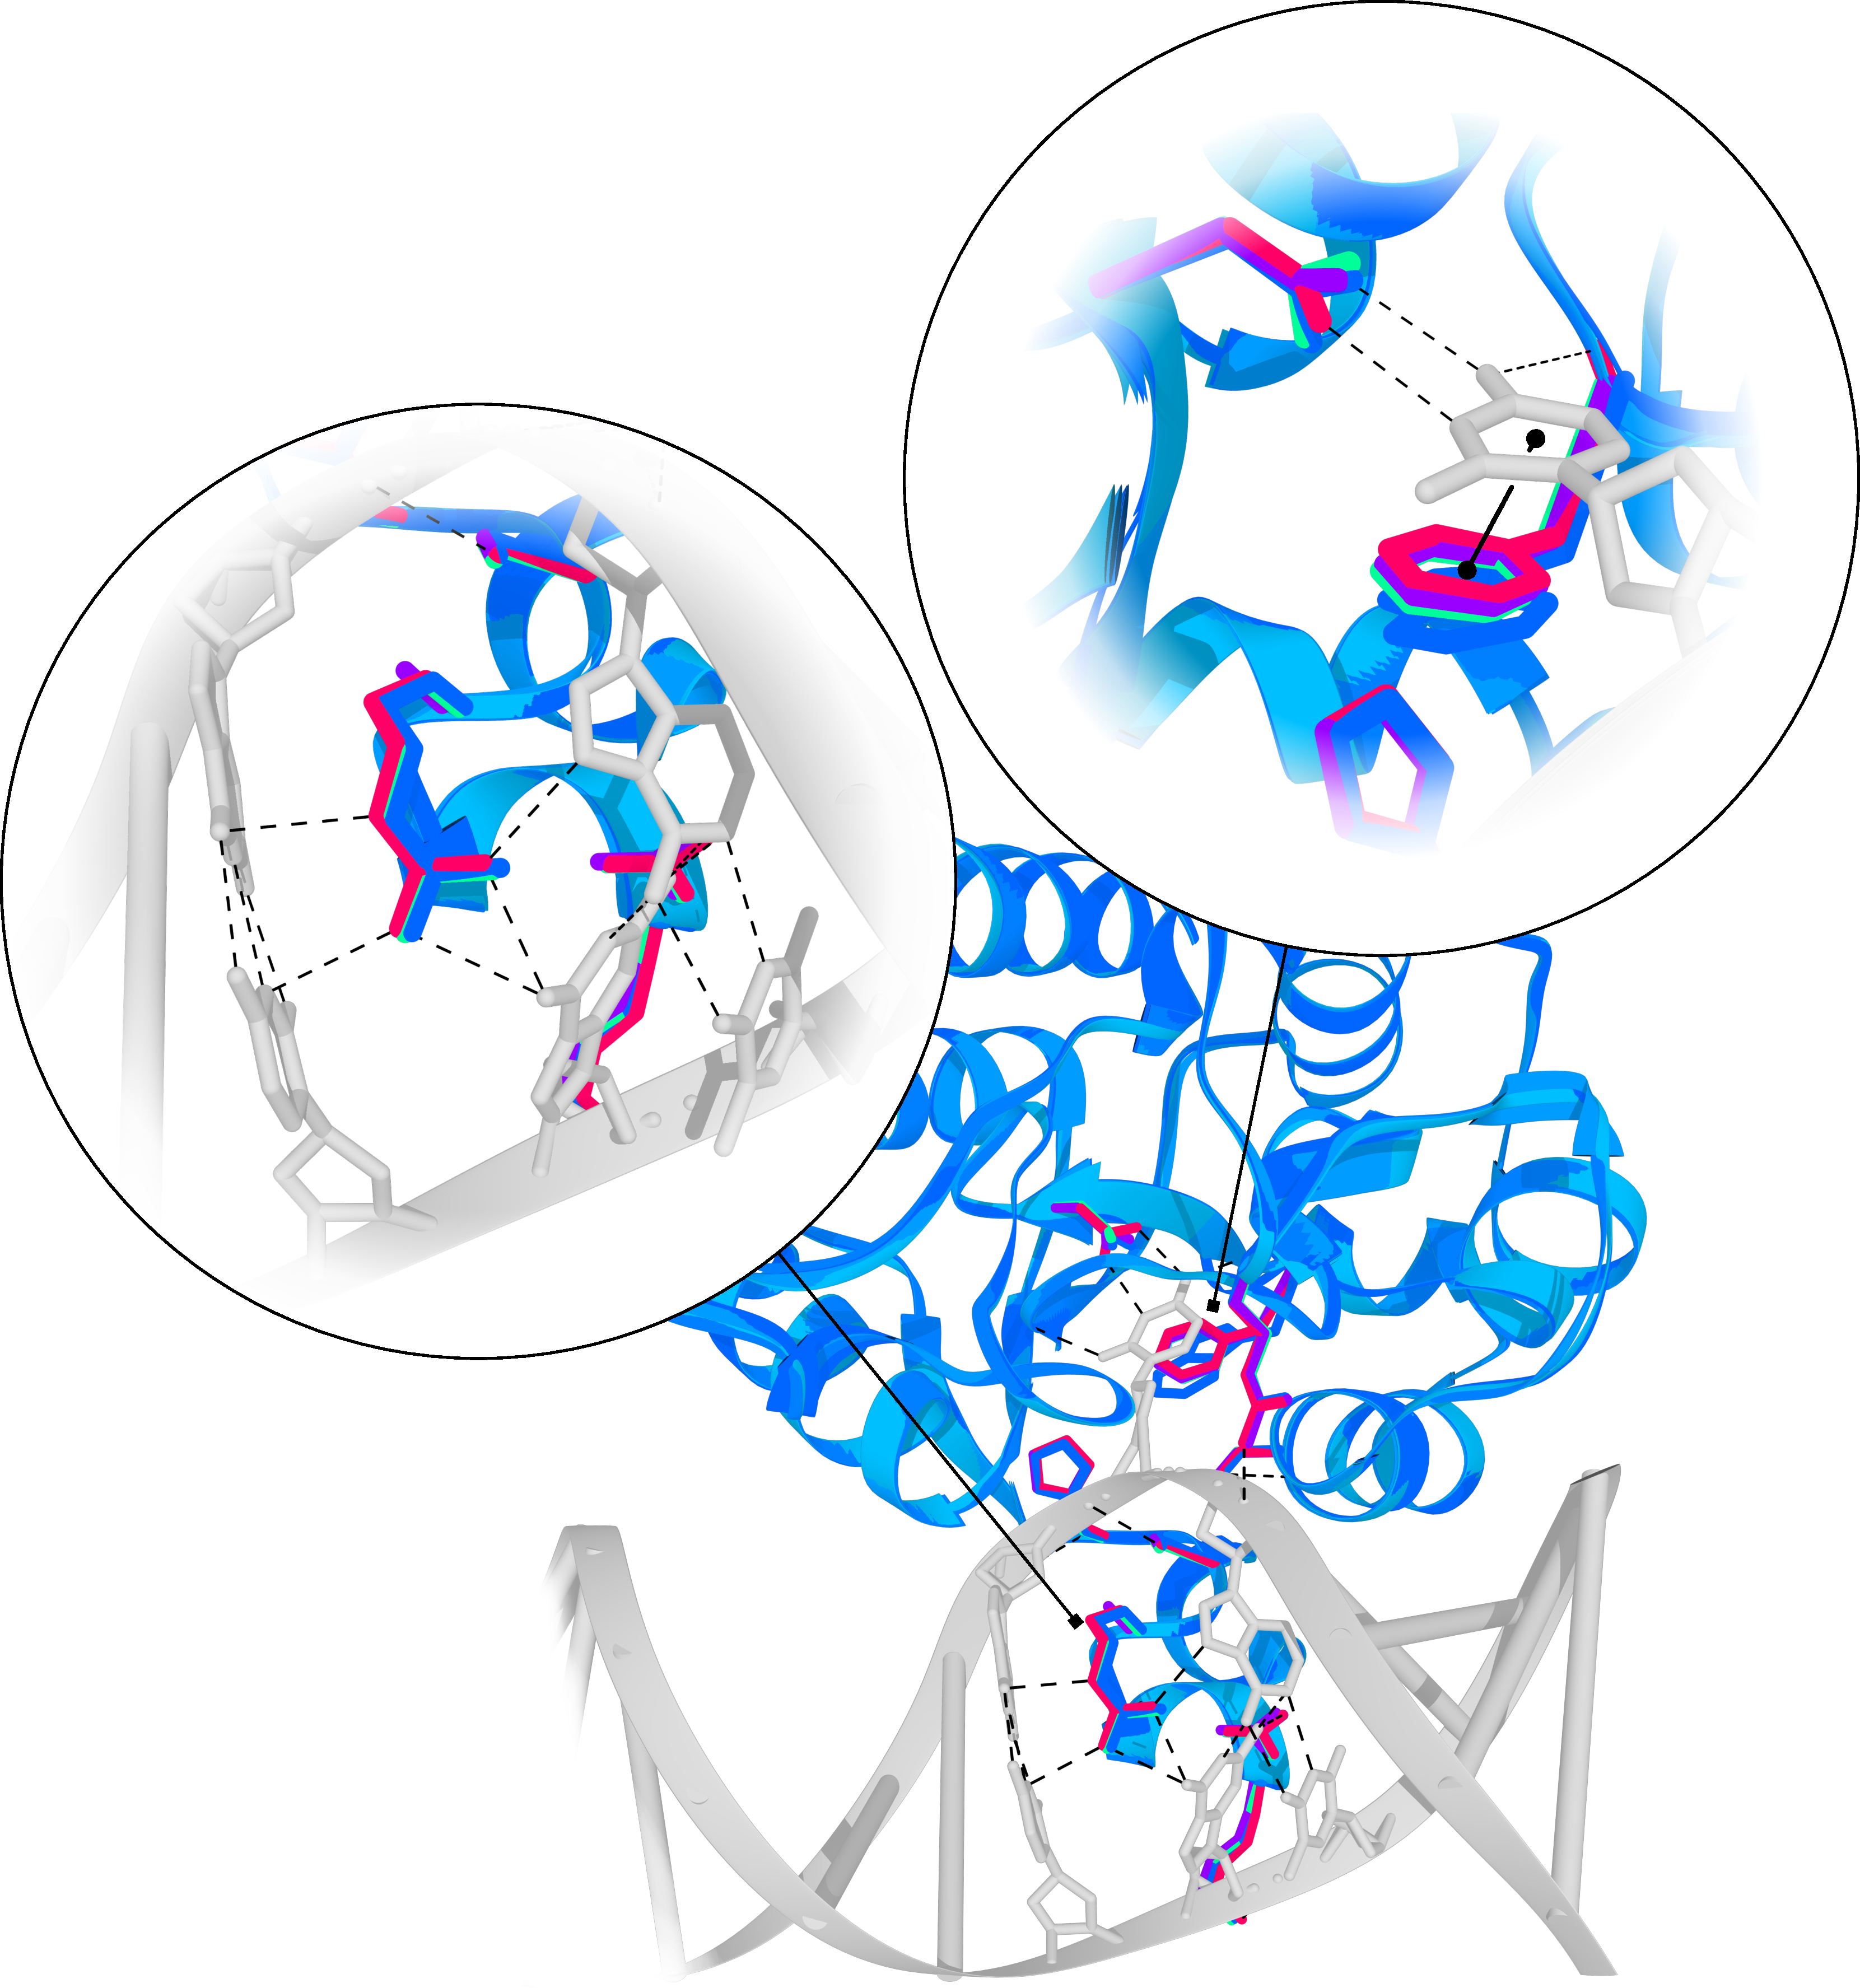
\includegraphics[width=.8\linewidth]{Guide/Figures/Protein.pdf}
  \caption{1b}
  \label{fig:sfig2}
\end{subfigure}
\begin{subfigure}{.5\textwidth}
  \centering
  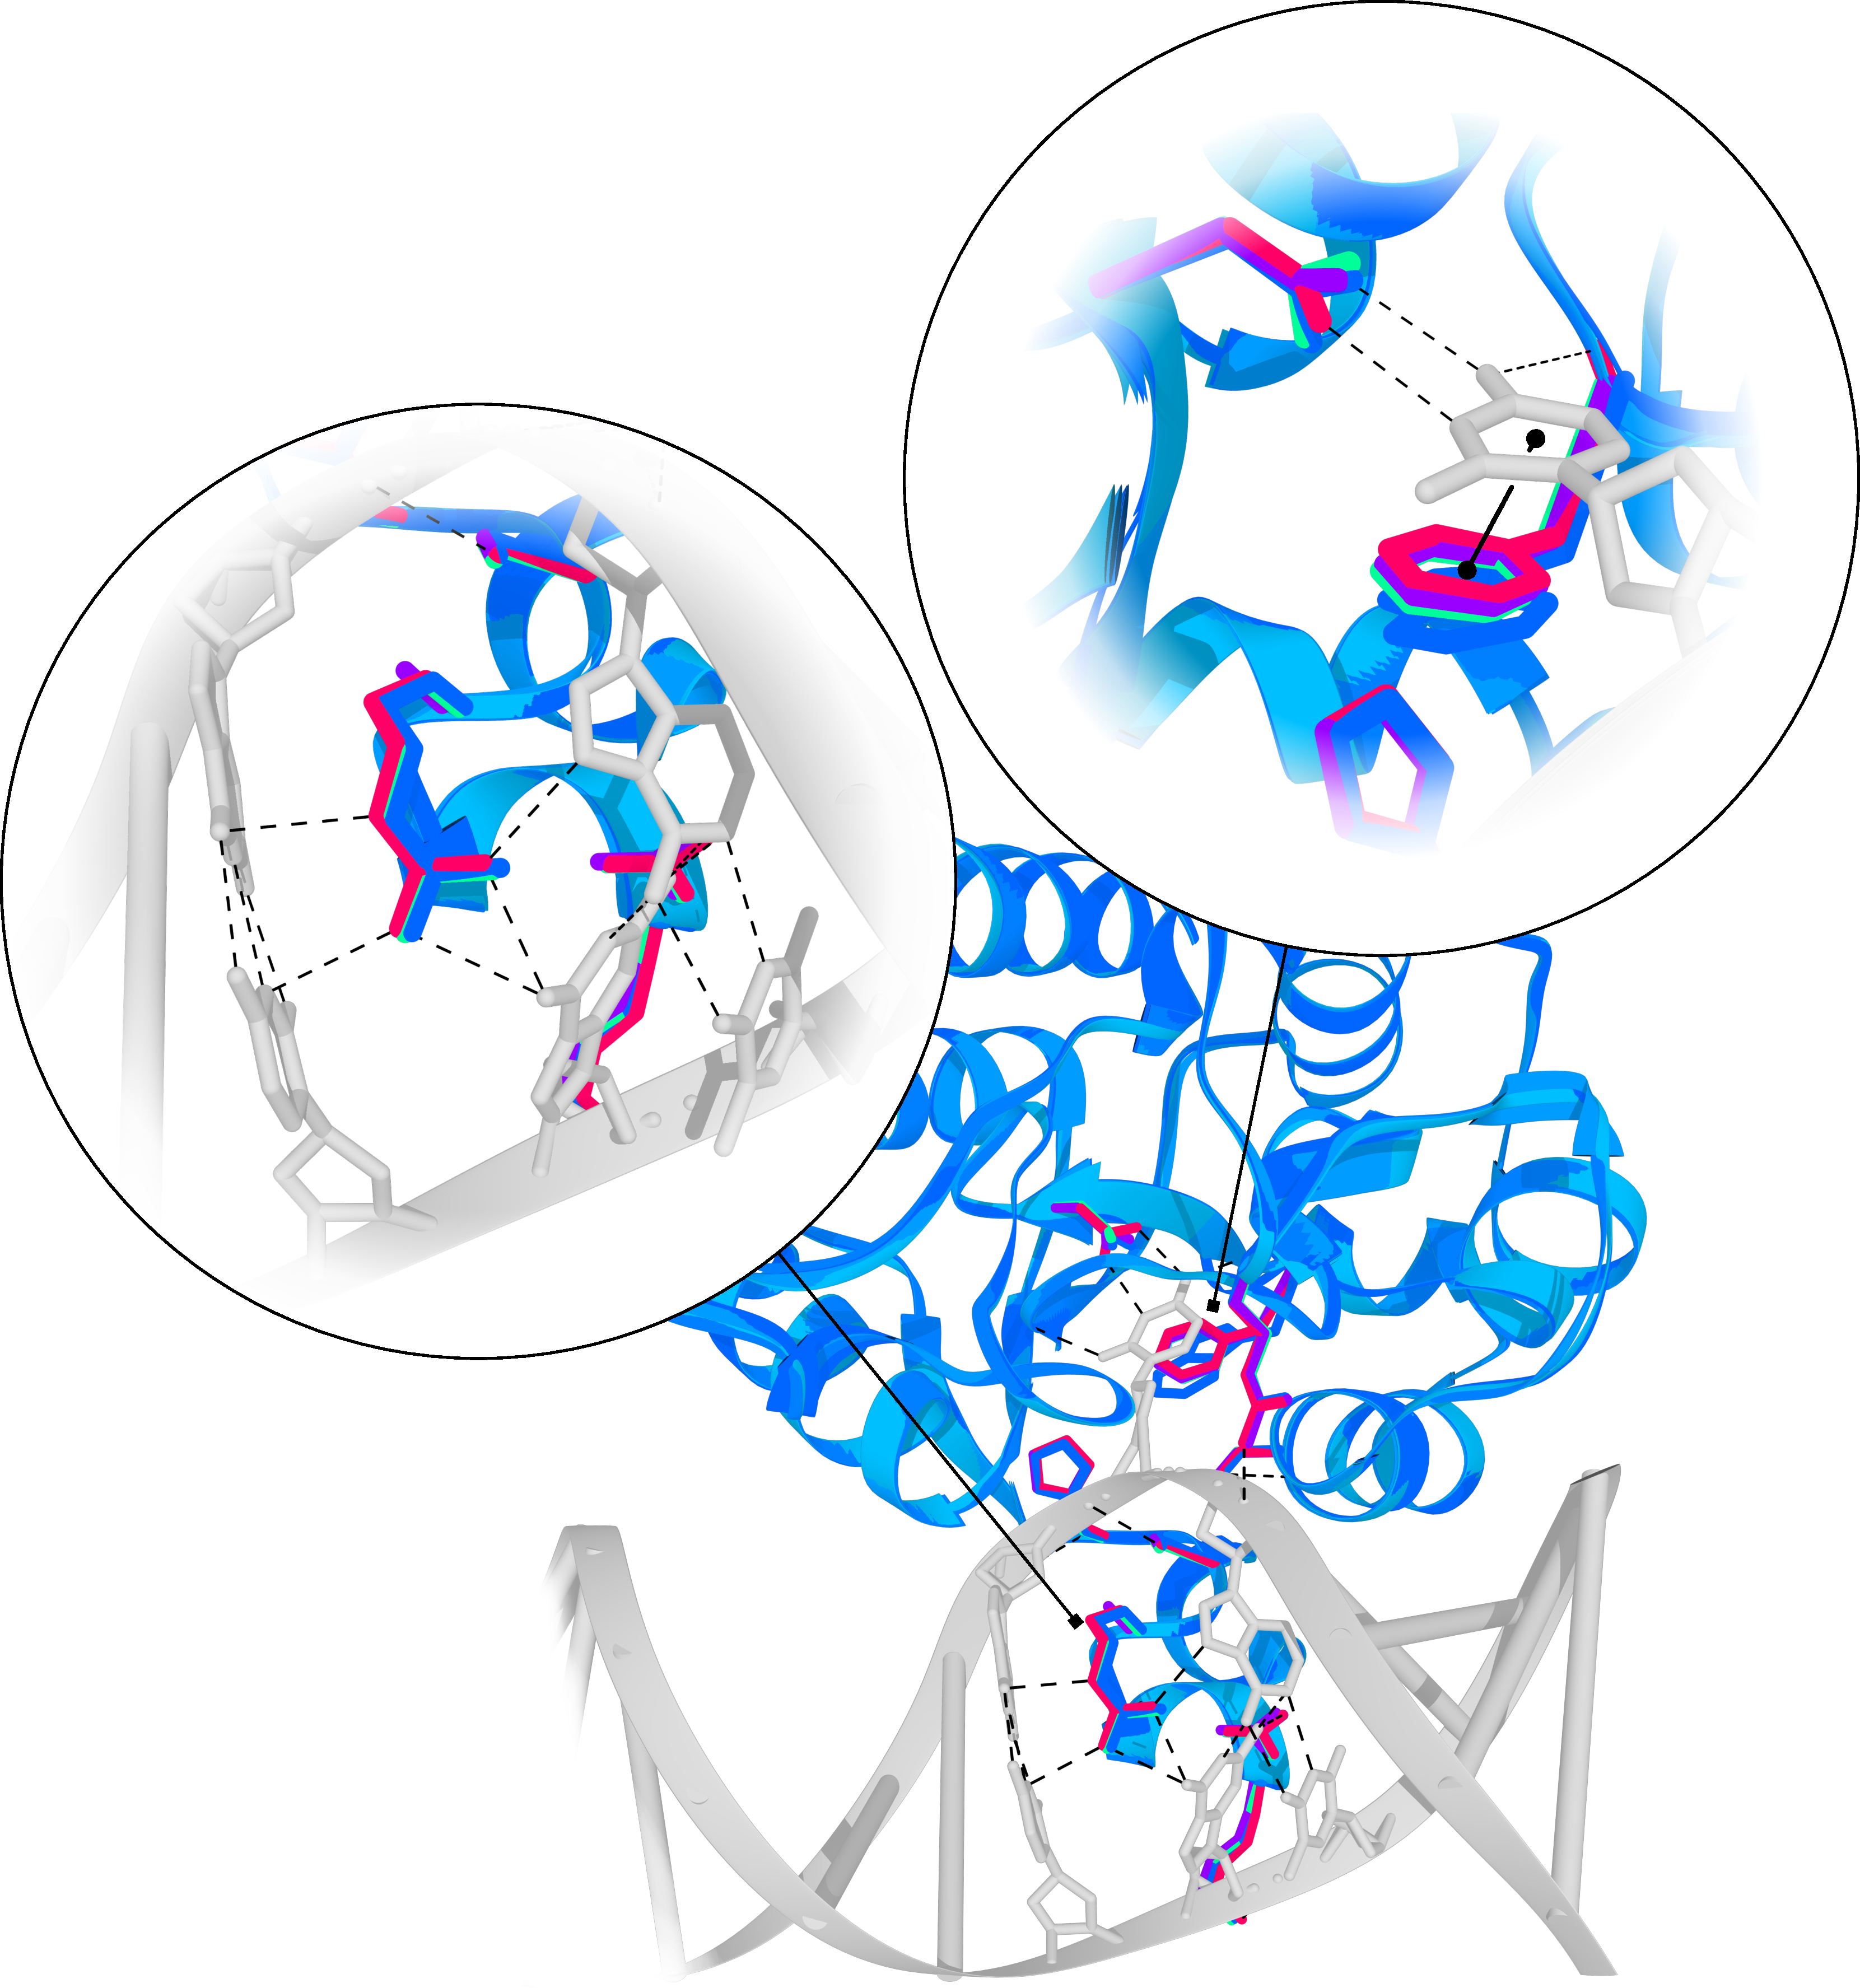
\includegraphics[width=.8\linewidth]{Guide/Figures/Protein.pdf}
  \caption{1b}
  \label{fig:sfig2}
\end{subfigure}
\caption{plots of....}
\label{fig:fig}
\end{figure}
